\documentclass{article}
\usepackage{graphicx, verbatim, kotex} % Required for inserting images


\title{[YACC-PL{1}]}
\author{형진 전}
\date{May 2024}

\begin{document}

\maketitle{}

\section{Introduction of YACC}
\subsection{YACC}
YACC는 유닉스 시스템의 표준 파서 생성기이며 흔히 syntax analyzer로 알려져 있다. 우리가 작성하는 코드가 컴퓨터에 입력될 때는 하나의 긴 문자열로 입력된다. Lex(Lexical Analyzer - 어휘분석기)가 이 긴 문자열로 된 코드를 정규표현식(Regular Expression)을 확인해 일정 문자열을 컴퓨터가 이해하는 숫자인 토큰으로 변환한다. YACC(Syntax Analyzer - 문법분석기)는 Lex가 변환한 토큰들을 가져와 문법을 확인한다. 문법이 오류 없이 시작 문법으로 변환된다면 그 코드는 오류가 없다는 것을 확인할 수 있다. 

\subsection{YACC의 Parsing}
YACC와 같은 구문 분석기는 BNF와 같은 의미 형식을 이용해 parsing tree를 만든다. parsing tree에는 크게 하향식과 상향식이 있다. 하향식은 root에 시작하는 파싱 방법으로 최좌단 전개와 상응한다. 최좌단 전개에 상응하게끔 토큰에 대한 맞는 RHS, 정의를 선택한다. 반대로 상향식은 leaf에서 시작해서 root까지 전개하는 방식으로 문자열들이 특정 LHS의 정의인 RHS로 귀결되게끔 하는 방식이다. 

\subsection{YACC의 구조}
YACC는 Lex와 같이 정의절, 규칙절, 서브루틴절로 이루어져 있다. 정의절에서는 Lex에서 받은 토큰들을 정의하고 오류를 확인할 수 있는 시작 문법으로 정의한다. 규칙절에서는 받은 토큰을 가지고 변환할 수 있는 문법을 정의한다. 마지막으로 서브루틴절은 문법을 변환할 때 수행해야 하는 특수한 조건들을 서브루틴의 형태로 선언해 놓은 곳이다. 예를 들면, yyerror()가 있다. 

\subsection{YACC의 작동 원리}
YACC는 Lex에서 받은 토큰들을 자료구조인 stack에 저장한다. stack에 들어온 토큰들이 문법에 맞게 된다면, stack의 내용과 입력을 받아 상태 전이를 일으킨다. 상태 전이가 일어나는 곳을 상태 기계(State Machine)라 한다. 

\newpage

\section{Lex Code}

\begin{verbatim}
D                       [0-9]
L                       [a-zA-Z_]
H                       [a-fA-F0-9]
E                       [Ee][+-]?{D}+
FS                      (f|F|l|L)
IS                      (u|U|l|L)*

%{
#include <stdio.h>
#include <string.h>
#include "y.tab.h"

void count();
void comment();
int check_type(); 
int struct_sign = 0, idx = 0, check_bracket = 0;
char *type[100];

%}

%%
"#include"[ ]*<.+\.h>   { return(INCLUDE); }

[설명 1]
#include <> 형태의 전처리문을 토큰으로 처리하기 위한 지시어다. 
"#include" 은 include, [ ]은 빈칸을 의미하며 뒤의 *은 0번 이상을 의미한다. 
<은 그냥 문자, .+은 아무 문자가 1번이상 나와야 함을, \.은 그냥 점, 뒤의 h>도 그냥 문자를 의미한다.

"#define"[ ]*{L}+[ ]*{D}+\.*{D}* 	{ return(DEFINE); }

[설명 2]
#define 형태의 전처리문을 토큰으로 처리하기 위한 지시어다.
"#define"은 #define, [ ]은 빈칸을 의미하며 뒤의 *은 0번 이상을 의미한다.
{L}은 Lex 정의절에서 정의한 Letter(L [a-zA-Z_])을 의미하고 +는 1번 이상
나와야 한다는 의미이다. {D}는 정의절에서 정의한 Digit(D [0-9])을 의미한다.
이 역시 +로 1번 이상 나와야 한다는 의미이다. 뒤는 \. 문자 .과 {D} Digit가
각각 0번 이상 나와야 한다는 의미이다.


"/*"                    { comment(); }
"auto"                  { count(); return(AUTO); }
"break"                 { count(); return(BREAK); }
"case"                  { count(); return(CASE); }
"char"                  { count(); return(CHAR); }
"const"                 { count(); return(CONST); }
"continue"              { count(); return(CONTINUE); }
"default"               { count(); return(DEFAULT); }
"do"                    { count(); return(DO); }
"double"                { count(); return(DOUBLE); }
"else"                  { count(); return(ELSE); }
"enum"                  { count(); return(ENUM); }
"extern"                { count(); return(EXTERN); }
"float"                 { count(); return(FLOAT); }
"for"                   { count(); return(FOR); }
"goto"                  { count(); return(GOTO); }
"if"                    { count(); return(IF); }
"int"                   { count(); return(INT); }
"long"                  { count(); return(LONG); }
"register"              { count(); return(REGISTER); }
"return"                { count(); return(RETURN); }
"short"                 { count(); return(SHORT); }
"signed"                { count(); return(SIGNED); }
"sizeof"                { count(); return(SIZEOF); }
"static"                { count(); return(STATIC); }
"struct"                { count(); struct_sign = 1; return(STRUCT); }

[설명 3] 
struct 구문이 나왔을 때 struct 뒤의 type_name을 감지하기 위해서 struct_sign이라는 변수를 설정하고 값을 1로 바꾸라는 명령이다.

"switch"                { count(); return(SWITCH); }
"typedef"               { count(); return(TYPEDEF); }
"union"                 { count(); return(UNION); }
"unsigned"              { count(); return(UNSIGNED); }
"void"                  { count(); return(VOID); }
"volatile"              { count(); return(VOLATILE); }
"while"                 { count(); return(WHILE); }
"else if"		        { return(ELIF); }

[설명 4]
else if 구문이 나왔을 때 if 구문으로 오해해 뒤의 YACC에서 중복해서 세지 말라고 특별히 넣은 토큰이다. Lex는 else if 문장을 발견하면 ELIF 이라는 토큰으로 변환한다.

{L}({L}|{D})*           { count(); return(check_type()); }

0[xX]{H}+{IS}?          { count(); return(CONSTANT); }
0{D}+{IS}?              { count(); return(CONSTANT); }
{D}+{IS}?               { count(); return(CONSTANT); }
L?'(\\.|[^\\'])+'       { count(); return(CONSTANT); }

{D}+{E}{FS}?            { count(); return(CONSTANT); }
{D}*"."{D}+({E})?{FS}?  { count(); return(CONSTANT); }
{D}+"."{D}*({E})?{FS}?  { count(); return(CONSTANT); }

L?\"(\\.|[^\\"])*\"     { count(); return(STRING_LITERAL); }

"..."                   { count(); return(ELLIPSIS); }
">>="                   { count(); return(RIGHT_ASSIGN); }
"<<="                   { count(); return(LEFT_ASSIGN); }
"+="                    { count(); return(ADD_ASSIGN); }
"-="                    { count(); return(SUB_ASSIGN); }
"*="                    { count(); return(MUL_ASSIGN); }
"/="                    { count(); return(DIV_ASSIGN); }
"%="                    { count(); return(MOD_ASSIGN); }
"&="                    { count(); return(AND_ASSIGN); }
"^="                    { count(); return(XOR_ASSIGN); }
"|="                    { count(); return(OR_ASSIGN); }
">>"                    { count(); return(RIGHT_OP); }
"<<"                    { count(); return(LEFT_OP); }
"++"                    { count(); return(INC_OP); }
"--"                    { count(); return(DEC_OP); }
"->"                    { count(); return(PTR_OP); }
"&&"                    { count(); return(AND_OP); }
"||"                    { count(); return(OR_OP); }
"<="                    { count(); return(LE_OP); }
">="                    { count(); return(GE_OP); }
"=="                    { count(); return(EQ_OP); }
"!="                    { count(); return(NE_OP); }
";"                     { count(); return(';'); }
("{"|"<%")              { count(); check_bracket = 1; return('{'); }
("}"|"%>")              { count(); check_bracket = 0; return('}'); }

[설명 5]
check_bracket은 struct에서 IDENTIFIER와 TYPE_NAME을 판단하기 위해 만든 변수이다.

","                     { count(); return(','); }
":"                     { count(); return(':'); }
"="                     { count(); return('='); }
"("                     { count(); return('('); }
")"                     { count(); return(')'); }
("["|"<:")              { count(); return('['); }
("]"|":>")              { count(); return(']'); }
"."                     { count(); return('.'); }
"&"                     { count(); return('&'); }
"!"                     { count(); return('!'); }
"~"                     { count(); return('~'); }
"-"                     { count(); return('-'); }
"+"                     { count(); return('+'); }
"*"                     { count(); return('*'); }
"/"                     { count(); return('/'); }
"%"                     { count(); return('%'); }
"<"                     { count(); return('<'); }
">"                     { count(); return('>'); }
"^"                     { count(); return('^'); }
"|"                     { count(); return('|'); }
"?"                     { count(); return('?'); }
"//"			        { /* ignore */ }

[설명 6]
"//" 라는 주석을 감지하기 위해 만든 구절이다. 밑의 "/*"의 주석을 감지하는 것과 같이 토큰을 감지하면 무시하라는 의미로 아무 것도 넣지 않고 만든 규칙이다.

[ \t\v\n\f]             { count(); }
.                       { /* ignore bad characters */ }

%%

int yywrap(){
        return 1;
}

void comment(){
        char c, c1;
loop:
        while((c = input()) != '*' && c != 0)
                putchar(c);
        if ((c1 = input()) != '/' && c != 0)
        {
                unput(c1);
                goto loop;
        }

        if (c != 0)
                putchar(c1);
}

int column = 0;

void count()
{
        int i;
        for(i = 0; yytext[i] != '\0'; i++)
                if (yytext[i] == '\n')
                        column = 0;
                else if (yytext[i] == '\t')
                        column += 8 - (column % 8);
                else
                        column++;

        ECHO;
}

int check_type()
{
	/*
        1-1. struct_sign == 1 검사하기.
        2-1. yytext를 char *type에 넣기.

        1-2. struct_sign == 0이라면, type안에 있는 타입인지 검사하기.
                - 문자열이 같다는 것을 확인하기
        2-2 값이 있으면 type_name 값을,
        2-3 값이 없으면 IDENTIFIER을 반환함.
        */
        
        
        if(struct_sign == 1 && check_bracket == 0) {
//printf("yes!1");
                type[idx] = yytext;
                idx++;
                struct_sign = 0;
                return(IDENTIFIER);
        } else {
//printf("yes!2");
                if(idx == 0) return(IDENTIFIER); 
//printf("yes!3");
                for(int i=0; i<=idx; i++) {
                        if(strcmp(yytext, type[i]) == 0) {
                                return(TYPE_NAME);
                        }
                }
                return(IDENTIFIER);        
        }        
        
}

[설명 7]

int check_type()은 struct에서 IDENTIFIER와 TYPE_NAME을 감지해 내기 위해 수정한 부분이다. struct을 처음 정의한 부분 뒤에 나오는 IDENTIFIER는 IDENTIFIER가 맞고, 더 나오는 경우를 대비하여 char *type[100]이라는 포인터 배열에 넣어야 한다. 후에 똑같은 yytext의 문자열이 나온다면 type에 들어있는 IDENTIFIER들과 비교하고 똑같은 문자열이 나온다면 이는 TYPE_NAME이라는 토큰으로 반환한다.

\end{verbatim}

\newpage

\section{YACC Code}
\begin{verbatim}
%{
#include <stdio.h>
int yylex();
void yyerror(const char* str);
int ary[9] = {0,0,0,0,0,0,0,0,0};
int id_cnt = 0;
int check_int = 0, check_char = 0;
int int_cnt =0, int_char = 0;
int buffer = 0;
#define YYDEBUG 1
%}

%token IDENTIFIER CONSTANT STRING_LITERAL SIZEOF
%token PTR_OP INC_OP DEC_OP LEFT_OP RIGHT_OP LE_OP GE_OP EQ_OP NE_OP
%token AND_OP OR_OP MUL_ASSIGN DIV_ASSIGN MOD_ASSIGN ADD_ASSIGN
%token SUB_ASSIGN LEFT_ASSIGN RIGHT_ASSIGN AND_ASSIGN
%token XOR_ASSIGN OR_ASSIGN TYPE_NAME

%token TYPEDEF EXTERN STATIC AUTO REGISTER
%token CHAR SHORT INT LONG SIGNED UNSIGNED FLOAT DOUBLE CONST VOLATILE VOID
%token STRUCT UNION ENUM ELLIPSIS

%token CASE DEFAULT IF ELSE SWITCH WHILE DO FOR GOTO CONTINUE BREAK RETURN INCLUDE DEFINE ELIF

%start translation_unit
%%

primary_expression
        : IDENTIFIER
        | CONSTANT
        | STRING_LITERAL
        | '(' expression ')'
        ;

postfix_expression
        : primary_expression
        | postfix_expression '[' expression ']'
        | postfix_expression '(' ')'
        | postfix_expression '(' argument_expression_list ')' { ary[0]++; }
        | postfix_expression '.' IDENTIFIER
        | postfix_expression PTR_OP IDENTIFIER
        | postfix_expression INC_OP { ary[1]++; }
        | postfix_expression DEC_OP { ary[1]++; }
        ;

argument_expression_list
        : assignment_expression
        | argument_expression_list ',' assignment_expression
        ;

unary_expression
        : postfix_expression
        | INC_OP unary_expression { ary[1]++; }
        | DEC_OP unary_expression { ary[1]++; }
        | unary_operator cast_expression
        | SIZEOF unary_expression
        | SIZEOF '(' type_name ')'
        ;

unary_operator
        : '&'
        | '*'
        | '+'
        | '-'
        | '~'
        | '!'
        ;
cast_expression
        : unary_expression
        | '(' type_name ')' cast_expression { ary[1]++; }
        ;

multiplicative_expression
        : cast_expression
        | multiplicative_expression '*' cast_expression { ary[1]++; }
        | multiplicative_expression '/' cast_expression { ary[1]++; }
        | multiplicative_expression '%' cast_expression { ary[1]++; }
        ;

additive_expression
        : multiplicative_expression
        | additive_expression '+' multiplicative_expression { ary[1]++; }
        | additive_expression '-' multiplicative_expression { ary[1]++; }
        ;

shift_expression
        : additive_expression
        | shift_expression LEFT_OP additive_expression { ary[1]++; }
        | shift_expression RIGHT_OP additive_expression { ary[1]++; }
        ;

relational_expression
        : shift_expression
        | relational_expression '<' shift_expression { ary[1]++; }
        | relational_expression '>' shift_expression { ary[1]++; }
        | relational_expression LE_OP shift_expression { ary[1]++; }
        | relational_expression GE_OP shift_expression { ary[1]++; }
        ;

equality_expression
        : relational_expression
        | equality_expression EQ_OP relational_expression { ary[1]++; }
        | equality_expression NE_OP relational_expression { ary[1]++; }
        ;

and_expression
        : equality_expression
        | and_expression '&' equality_expression { ary[1]++; }
        ;

exclusive_or_expression
        : and_expression
        | exclusive_or_expression '^' and_expression { ary[1]++; }
        ;

inclusive_or_expression
        : exclusive_or_expression
        | inclusive_or_expression '|' exclusive_or_expression { ary[1]++; }
        ;

logical_and_expression
        : inclusive_or_expression
        | logical_and_expression AND_OP inclusive_or_expression { ary[1]++; }
        ;


logical_or_expression
        : logical_and_expression
        | logical_or_expression OR_OP logical_and_expression { ary[1]++; }
        ;

conditional_expression
        : logical_or_expression
        | logical_or_expression '?' expression ':' conditional_expression
        ;

assignment_expression
        : conditional_expression
        | unary_expression assignment_operator assignment_expression
        ;

assignment_operator
        : '=' { ary[1]++; }
        | MUL_ASSIGN { ary[1]++; }
        | DIV_ASSIGN { ary[1]++; }
        | MOD_ASSIGN { ary[1]++; }
        | ADD_ASSIGN { ary[1]++; }
        | SUB_ASSIGN { ary[1]++; }
        | LEFT_ASSIGN { ary[1]++; }
        | RIGHT_ASSIGN { ary[1]++; }
        | AND_ASSIGN { ary[1]++; }
        | XOR_ASSIGN { ary[1]++; }
        | OR_ASSIGN { ary[1]++; }
        ;

expression
        : assignment_expression
        | expression ',' assignment_expression
        ;

constant_expression
        : conditional_expression
        ;

declaration
        : declaration_specifiers ';'
        | declaration_specifiers init_declarator_list ';' { if(check_int){ ary[2] += id_cnt; check_int = id_cnt = 0; } if(check_char){ ary[3] += id_cnt; check_char = id_cnt = 0; } }

declaration_specifiers
        : storage_class_specifier
        | storage_class_specifier declaration_specifiers
        | type_specifier
        | type_specifier declaration_specifiers
        | type_qualifier
        | type_qualifier declaration_specifiers
        ;

init_declarator_list
        : init_declarator 
        | init_declarator_list ',' init_declarator
        ;

// variables
init_declarator
        : declarator
        | declarator '=' initializer { ary[1]++; }
        ;

storage_class_specifier
        : TYPEDEF
        | EXTERN
        | STATIC
        | AUTO
        | REGISTER
        ;

type_specifier
        : VOID
        | CHAR { check_char = 1; buffer = 0; printf("pin_check_char\n"); }
	| SHORT
        | INT { check_int = 1; buffer = 1; printf("pin_check_int\n"); }
        | LONG
        | FLOAT
        | DOUBLE
        | SIGNED
        | UNSIGNED
        | struct_or_union_specifier
        | enum_specifier
        | TYPE_NAME
        ;

struct_or_union_specifier
        : struct_or_union IDENTIFIER '{' struct_declaration_list '}'
        | struct_or_union '{' struct_declaration_list '}'	
        | struct_or_union IDENTIFIER
        ;

struct_or_union
        : STRUCT
        | UNION
        ;

struct_declaration_list
        : struct_declaration
        | struct_declaration_list struct_declaration
        ;

struct_declaration
        : specifier_qualifier_list struct_declarator_list ';'
        ;

specifier_qualifier_list
        : type_specifier specifier_qualifier_list
        | type_specifier
        | type_qualifier specifier_qualifier_list
        | type_qualifier
        ;

struct_declarator_list
        : struct_declarator
        | struct_declarator_list ',' struct_declarator
        ;

struct_declarator
        : declarator
        | ':' constant_expression
        | declarator ':' constant_expression
        ;

enum_specifier
        : ENUM '{' enumerator_list '}'
        | ENUM IDENTIFIER '{' enumerator_list '}'
        | ENUM IDENTIFIER
        ;

enumerator_list
        : enumerator
        | enumerator_list ',' enumerator
        ;

enumerator
        : IDENTIFIER
        | IDENTIFIER '=' constant_expression
        ;

type_qualifier
        : CONST
        | VOLATILE
        ;

declarator
        : pointer direct_declarator { ary[4]++; }
        | direct_declarator
        ;

direct_declarator
        : IDENTIFIER { id_cnt++; }
        | '(' declarator ')'
        | direct_declarator '[' constant_expression ']' { ary[5]++; } 
        | direct_declarator '[' ']' { ary[5]++; }
        | direct_declarator '(' parameter_type_list ')' { id_cnt = 0; check_int = check_char = 0; printf("pin_zerop\n"); ary[0]++; }
        | direct_declarator '(' identifier_list ')' { id_cnt = 0; check_int = check_char = 0; printf("pin_zeroi\n"); ary[0]++; }
        | direct_declarator '(' ')' { id_cnt = 0; check_int = check_char = 0; printf("pin_zero\n"); ary[0]++; } 
        ;

pointer
        : '*' 
        | '*' type_qualifier_list
        | '*' pointer
        | '*' type_qualifier_list pointer
        ;

type_qualifier_list
        : type_qualifier
        | type_qualifier_list type_qualifier
	;

parameter_type_list
        : parameter_list 
        | parameter_list ',' ELLIPSIS
        ;

parameter_list
        : parameter_declaration
        | parameter_list ',' parameter_declaration
        ;


parameter_declaration
        : declaration_specifiers declarator { if(buffer){ ary[2]++; }else{ ary[3]++; } } 
        | declaration_specifiers abstract_declarator
        | declaration_specifiers
        ;

identifier_list
        : IDENTIFIER
        | identifier_list ',' IDENTIFIER
        ;

type_name
        : specifier_qualifier_list
        | specifier_qualifier_list abstract_declarator
        ;

abstract_declarator
        : pointer
        | direct_abstract_declarator
        | pointer direct_abstract_declarator
        ;

direct_abstract_declarator
        : '(' abstract_declarator ')'
        | '[' ']' 
        | '[' constant_expression ']'
        | direct_abstract_declarator '[' ']'
        | direct_abstract_declarator '[' constant_expression ']'
        | '(' ')'
        | '(' parameter_type_list ')'
        | direct_abstract_declarator '(' ')'
        | direct_abstract_declarator '(' parameter_type_list ')'
        ;

initializer
        : assignment_expression
        | '{' initializer_list '}'
       	| '{' initializer_list ',' '}'
        ;

initializer_list
        : initializer
        | initializer_list ',' initializer
        ;

statement
     	: labeled_statement
        | compound_statement
        | expression_statement
        | selection_statement
        | iteration_statement
        | jump_statement
        ;

labeled_statement
        : IDENTIFIER ':' statement
        | CASE constant_expression ':' statement
        | DEFAULT ':' statement
        ;

compound_statement
        : '{' '}'
        | '{' statement_list '}'
        | '{' declaration_list '}'
        | '{' declaration_list statement_list '}'
        ;

declaration_list
        : declaration
        | declaration_list declaration
        | declaration_list statement_list
        ;

statement_list
        : statement
        | statement_list statement
        ;

expression_statement
        : ';'
        | expression ';'
        ;

selection_statement
        : IF '(' expression ')' statement { ary[6]++; }
        | IF '(' expression ')' statement ELSE statement { ary[6]++; } 
        | ELIF '(' expression ')' statement 
        | ELIF '(' expression ')' statement ELSE statement 
        | SWITCH '(' expression ')' statement { ary[6]++; }
        ;

iteration_statement
        : WHILE '(' expression ')' statement { ary[7]++; }
        | DO statement WHILE '(' expression ')' ';' { ary[7]++; }
        | FOR '(' expression_statement expression_statement ')' statement { ary[7]++; }
        | FOR '(' expression_statement expression_statement expression ')' statement { ary[7]++; }
        | FOR '(' declaration expression_statement expression ')' statement { ary[7]++; }
        ;

jump_statement
        : GOTO IDENTIFIER ';'
        | CONTINUE ';'
        | BREAK ';'
        | RETURN ';' { ary[8]++; }
        | RETURN expression ';' { ary[8]++; }
        ;

header
        : INCLUDE
        | DEFINE
        | header INCLUDE
        | header DEFINE 
        ;

translation_unit
        : external_declaration
        | header external_declaration
        | translation_unit external_declaration
        ;

external_declaration
        : function_definition  
        | declaration
        ;

function_definition
        : declaration_specifiers declarator declaration_list compound_statement
        | declaration_specifiers declarator compound_statement
        | declarator declaration_list compound_statement
        | declarator compound_statement
        ;



%%

int main(void)
{
        #if YYDEBUG
                yydebug = 1;
        #endif
        yyparse();
        printf("function = %d\n", ary[0]);
        printf("operator = %d\n", ary[1]);
        printf("int = %d\n", ary[2]);
        printf("char = %d\n", ary[3]);
        printf("pointer = %d\n", ary[4]);
        printf("array = %d\n", ary[5]);
        printf("selection = %d\n", ary[6]);
        printf("loop = %d\n", ary[7]);
        printf("return = %d\n", ary[8]);
        return 0;
}


void yyerror(const char * str){
        fprintf(stderr, "error : %s\n", str);
}





\end{verbatim}

\newpage

\subsection{include, define}
\begin{figure}[h]
    \centering
    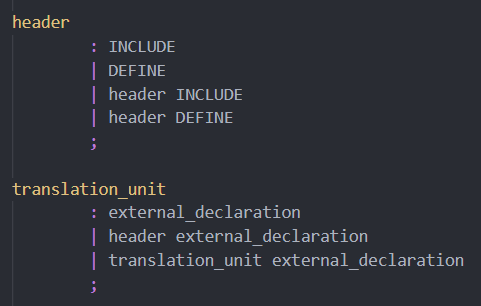
\includegraphics[scale = 0.8]{header define.png}
    \caption{Caption}
\end{figure}

Lex에서 받아온 토큰 중 INCLUDE와 DEFINE 토큰을 정리하기 위해 규칙절에 header에 관한 규칙을 추가했다. 둘을 모두 header 상태로 전이한다. #include와 #define이 중복해서 나올 경우를 대비해 'header INCLUDE', 'header DEFINE' 규칙으로 right recursive로 정리한 모습이다. header에 대한 정리가 끝났다면 밑의 translation unit에서 'header external\_declaration'으로 전이한다.

\subsection{statement}
\begin{figure}[h]
    \centering
    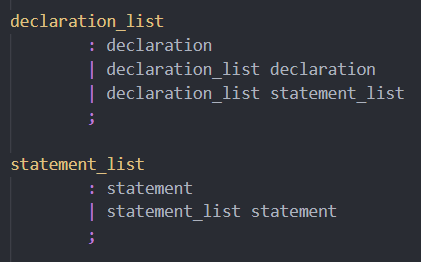
\includegraphics[scale = 0.8]{statement.png}
    \caption{Caption}
\end{figure}

'i=0'; 중간에 선언문이 나와도 해결될 수 있게 'declaration\_list statement\_list' 규칙을 declaration\_list에 추가했다.

\newpage

\subsection{function}
\begin{figure}[h]
    \centering
    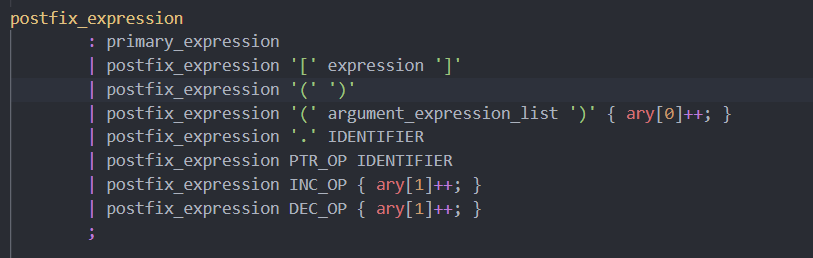
\includegraphics[scale = 0.8]{function1.png}
    \caption{Caption}
\end{figure}
postfix\_expression '(' argument\_expression\_list ')'은 printf와 scanf하는 내장 함수를 설정하는 부분으로 함수의 개수를 세는데 반드시 필요한 부분이다.

\begin{figure}[h]
    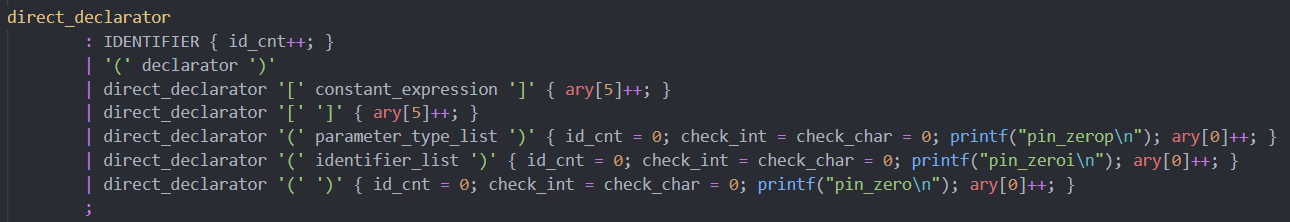
\includegraphics[scale = 0.63]{function2.png}
    \caption{Caption}
\end{figure}
direct\_declarator '(' parameter\_type\_list ')' { ary[0]++; }

direct\_declarator '(' identifier\_list ')' { ary[0]++; }

direct\_declarator '(' ')' { ary[0]++; } 

함수가 선언될 때 혹은 사용될 때 둘 중 한번 카운트가 되어야 한다. 이 코드에서는 사용될 때 카운트가 되도록 설정했다.

\newpage

\subsection{operation}
\begin{verbatim}
postfix_expression
        : primary_expression
        | postfix_expression '[' expression ']'
        | postfix_expression '(' ')'
        | postfix_expression '(' argument_expression_list ')' { ary[0]++; }
        | postfix_expression '.' IDENTIFIER
        | postfix_expression PTR_OP IDENTIFIER
        | postfix_expression INC_OP { ary[1]++; }
        | postfix_expression DEC_OP { ary[1]++; }
        ;

argument_expression_list
        : assignment_expression
        | argument_expression_list ',' assignment_expression
        ;

unary_expression
        : postfix_expression
        | INC_OP unary_expression { ary[1]++; }
        | DEC_OP unary_expression { ary[1]++; }
        | unary_operator cast_expression
        | SIZEOF unary_expression
        | SIZEOF '(' type_name ')'
        ;

unary_operator
        : '&'
        | '*'
        | '+'
        | '-'
        | '~'
        | '!'
        ;
cast_expression
        : unary_expression
        | '(' type_name ')' cast_expression { ary[1]++; }
        ;

multiplicative_expression
        : cast_expression
        | multiplicative_expression '*' cast_expression { ary[1]++; }
        | multiplicative_expression '/' cast_expression { ary[1]++; }
        | multiplicative_expression '%' cast_expression { ary[1]++; }
        ;

additive_expression
        : multiplicative_expression
        | additive_expression '+' multiplicative_expression { ary[1]++; }
        | additive_expression '-' multiplicative_expression { ary[1]++; }
        ;

shift_expression
        : additive_expression
        | shift_expression LEFT_OP additive_expression { ary[1]++; }
        | shift_expression RIGHT_OP additive_expression { ary[1]++; }
        ;

relational_expression
        : shift_expression
        | relational_expression '<' shift_expression { ary[1]++; }
        | relational_expression '>' shift_expression { ary[1]++; }
        | relational_expression LE_OP shift_expression { ary[1]++; }
        | relational_expression GE_OP shift_expression { ary[1]++; }
        ;

equality_expression
        : relational_expression
        | equality_expression EQ_OP relational_expression { ary[1]++; }
        | equality_expression NE_OP relational_expression { ary[1]++; }
        ;

and_expression
        : equality_expression
        | and_expression '&' equality_expression { ary[1]++; }
        ;

exclusive_or_expression
        : and_expression
        | exclusive_or_expression '^' and_expression { ary[1]++; }
        ;

inclusive_or_expression
        : exclusive_or_expression
        | inclusive_or_expression '|' exclusive_or_expression { ary[1]++; }
        ;

logical_and_expression
        : inclusive_or_expression
        | logical_and_expression AND_OP inclusive_or_expression { ary[1]++; }
        ;


logical_or_expression
        : logical_and_expression
        | logical_or_expression OR_OP logical_and_expression { ary[1]++; }
        ;

conditional_expression
        : logical_or_expression
        | logical_or_expression '?' expression ':' conditional_expression
        ;

assignment_expression
        : conditional_expression
        | unary_expression assignment_operator assignment_expression
        ;

assignment_operator
        : '=' { ary[1]++; }
        | MUL_ASSIGN { ary[1]++; }
        | DIV_ASSIGN { ary[1]++; }
        | MOD_ASSIGN { ary[1]++; }
        | ADD_ASSIGN { ary[1]++; }
        | SUB_ASSIGN { ary[1]++; }
        | LEFT_ASSIGN { ary[1]++; }
        | RIGHT_ASSIGN { ary[1]++; }
        | AND_ASSIGN { ary[1]++; }
        | XOR_ASSIGN { ary[1]++; }
        | OR_ASSIGN { ary[1]++; }
        ;
[설명]
연산자가 포함되는 모든 경우에 ary[1]++을 추가했다.


init_declarator
        : declarator
        | declarator '=' initializer { ary[1]++; }
        ;
[설명]
특히 마지막 부분은 변수 선언과 매개변수 선언시 초기화를 하는 경우에도 대입연산자를 사용하기 때문에 이 부분에도 ary[1]++ 부분을 추가했다. 

\end{verbatim}

\newpage

\subsection{int, char 갯수 세기}
\begin{verbatim}
int main()
main:
direct_declarator : IDENTIFIER
direct_declarator : direct_declarator()
declarator : direct_declarator
declaration_specifiers declarator declaration_list compound_statement
INT				main		()		{ declaration_list }

variables:
declarator : direct_declarator
init_declarator : declarator
init_declarator_list : init_declarator
declaration : declaration_specifiers init_declarator_list ';'
declaration_list : declaration

type_specifier
        : VOID
        | CHAR { check_char = 1; printf("pin_check_char\n"); }
        | SHORT
        | INT { check_int = 1; printf("pin_check_int\n"); }
        | LONG
        | FLOAT
        | DOUBLE
        | SIGNED
        | UNSIGNED
        | struct_or_union_specifier
        | enum_specifier
        | TYPE_NAME
        ;
:direct_declarator
        : IDENTIFIER { id_cnt++; }
        | '(' declarator ')'
        | direct_declarator '[' constant_expression ']'
        | direct_declarator '[' ']'
        | direct_declarator '(' parameter_type_list ')' { id_cnt--; }
        | direct_declarator '(' identifier_list ')' { id_cnt--; }
        | direct_declarator '(' ')' { id_cnt--; }
        ;
declaration
        : declaration_specifiers ';'
        | declaration_specifiers init_declarator_list ';' { if(check_int){ ary[2] += id_cnt; check_int = id_cnt = 0; } if(check_char){ ary[3] += id_cnt; check_char = id_cnt = 0; } }

int와 char의 갯수를 세는데 필요한 항목들이다. INT 와 CHAR 토큰은 따로 있어 분간하기 쉽지만, 각각의 변수들 그리고 세면 안되는 함수들은 같은 문법을 따라가는 경우가 있어 구별하기 어려웠다. 구현한 방법은 함수로 합쳐지는 direct_declarator의 함수 문법을 따르는 경우 identifier를 세는 총합 cnt 갯수에서 하나를 뺐다. 이 뜻은 int 아니면 char로 세어지는 함수의 갯수만큼 변수갯수에서 빼겠다는 의미이다.

이렇게 했더니 
int example (char a, char b);
함수 이름도 같은 IDENTIFIER이기 때문에 int와 char의 갯수에 함수 이름도 포함되어 버리는 현상이 발생했다. 함수 이름은 int와 char의 갯수에서 제외해야 하기 때문에 수정이 필요했다. 

type_specifier
        : VOID
        | CHAR { check_char = 1; buffer = 0; printf("pin_check_char\n"); }
        | SHORT
        | INT { check_int = 1; buffer = 1; printf("pin_check_int\n"); }
        | LONG
        | FLOAT
        | DOUBLE
        | SIGNED
        | UNSIGNED
        | struct_or_union_specifier
        | enum_specifier
        | TYPE_NAME
        ;

direct_declarator
        : IDENTIFIER { id_cnt++; }
        | '(' declarator ')'
        | direct_declarator '[' constant_expression ']'
        | direct_declarator '[' ']'
        | direct_declarator '(' parameter_type_list ')' { id_cnt = 0; check_int = check_char = 0; printf("pin_zerop\n"); ary[0]++; }
        | direct_declarator '(' identifier_list ')' { id_cnt = 0; check_int = check_char = 0; printf("pin_zeroi\n"); ary[0]++; }
        | direct_declarator '(' ')' { id_cnt = 0; check_int = check_char = 0; printf("pin_zero\n"); ary[0]++; }
        ;

declaration
        : declaration_specifiers ';'
        | declaration_specifiers init_declarator_list ';' 
        { if(check_int){ ary[2] += id_cnt; check_int = id_cnt = 0; }
        if(check_char){ ary[3] += id_cnt; check_char = id_cnt = 0; } }

parameter_declaration
        : declaration_specifiers declarator { if(buffer){ ary[2]++; }else{ ary[3]++; } }
        | declaration_specifiers abstract_declarator
        | declaration_specifiers
        ;

int buffer를 두어 함수 자료형과 파라미터 자료형이 다른 경우와 같은 경우를 구별했다. buffer는 int 나 char에 따라서 값이 바뀌게 되는데, 함수 자료형의 상관 없이 오직 파라미터의 자료형만 세어 int와 char의 갯수를 올려준다. 이렇게 하면 함수 자료형의 수와 파라미터 자료형의 수가 겹쳐지는 문제를 해결할 수 있다.

\end{verbatim}

\newpage

\subsection{pointer}
\begin{figure}[h]
    \centering
    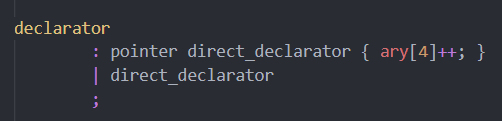
\includegraphics[scale = 0.8]{pointer.png}
    \caption{Caption}
\end{figure}
이 부분만 포인터의 갯수를 세면 이중포인터든 일반 포인터든 한번만 세게 된다.

\subsection{array}
\begin{figure}[h]
    \centering
    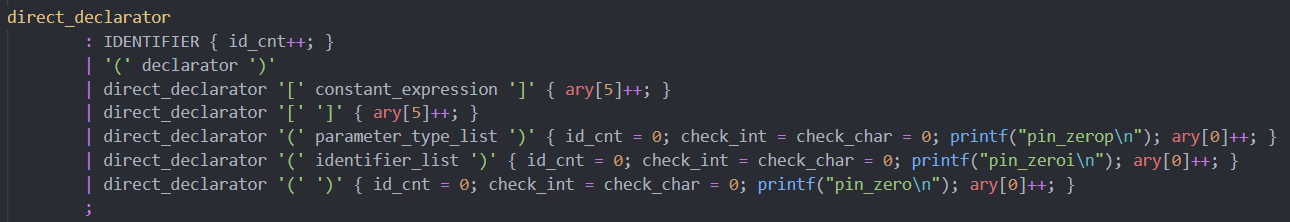
\includegraphics[scale = 0.8]{function2.png}
    \caption{Caption}
\end{figure}
direct\_declarator '[' constant\_expression ']' { ary[5]++; }

direct\_declarator '[' ']' { ary[5]++; }

direct\_declarator에 배열을 선언할 때 사용하는 규칙이 있다. 이걸 이용하면 배열의 갯수를 셀 수 있다.

\newpage

\subsection{selection}
\begin{figure}[h]
    \centering
    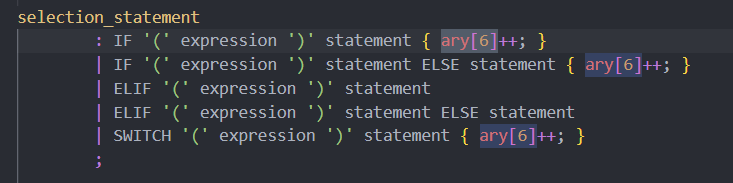
\includegraphics[scale = 0.8]{selection.png}
    \caption{selection}
\end{figure}
위의 lex에서 정의했단 ELIF token을 여기서 사용한다. 오직 IF와 SWITCH 토큰이 나오면 selection에 대한 갯수를 세고 나머진 세지 않는다.

\subsection{loop}
\begin{figure}[h]
    \centering
    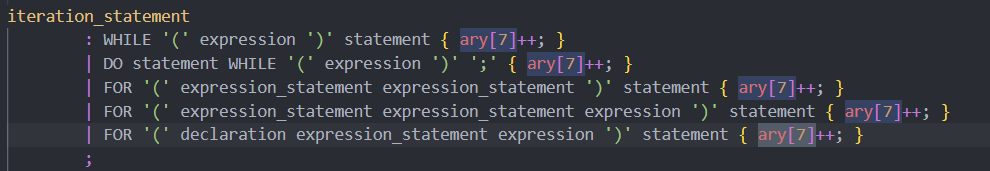
\includegraphics[scale = 0.8]{loop.png}
    \caption{loop}
\end{figure}
loop 관련 토큰이나 문법이 나오면 이 부분에서 전부 갯수를 센다.

\subsection{return}
\begin{figure}[h]
    \centering
    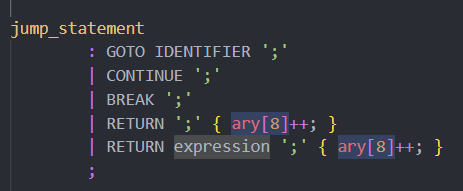
\includegraphics[scale = 0.8]{return.png}
    \caption{return}
\end{figure}
return 관련 토큰이나 문법이 나오면 이 부분에서 전부 갯수를 센다.

\end{document}
